% preamble-exam-zh.tex — 极简讲解页共享 preamble
% 目标：复刻「题目独立、提示轻框、路线箭头、主体双栏、答案轻收束」的讲义风格。

\documentclass{exam-zh}

% ---------- 基础配置 ----------
\examsetup{
  page/size = a4paper,
  page/show-head = false,
  page/show-foot = false,
  sealline/show = false,
  font = none,
  math-font = none,
}

% ---------- 包 ----------
\usepackage{geometry}
\geometry{top=10mm,bottom=14mm,left=12mm,right=10mm}
\AtBeginDocument{\newgeometry{top=10mm,bottom=14mm,left=12mm,right=10mm}}

\usepackage{xcolor}
\usepackage{needspace}
\usepackage{enumitem}
\usepackage{array}
\usepackage{tabularx}
\usepackage{tcolorbox}
\tcbuselibrary{skins,breakable}
\usepackage{paracol}

% ---------- 打印/屏幕颜色切换 ----------
% 用法：\documentclass[monochrome]{exam-zh} 可降级为灰度。
% 注意：不要使用 \if@xxx 放在 makeatother 外部；这里改成普通条件名。
\newif\ifeduprintcolor
\eduprintcolortrue
\makeatletter
\@ifclasswith{exam-zh}{monochrome}{\eduprintcolorfalse}{}
\makeatother

% ---------- 语义颜色 ----------
\ifeduprintcolor
  \definecolor{edu-blue}{RGB}{31,62,126}
  \definecolor{edu-blue-soft}{RGB}{232,238,250}
  \definecolor{edu-blue-bg}{RGB}{248,250,254}
  \definecolor{edu-ink}{RGB}{30,35,45}
  \definecolor{edu-muted}{RGB}{118,124,136}
  \definecolor{edu-line}{RGB}{209,218,235}
  \definecolor{edu-soft-bg}{RGB}{250,251,253}
  \definecolor{edu-red}{RGB}{168,58,58}
  \definecolor{edu-red-bg}{RGB}{255,247,245}
\else
  \definecolor{edu-blue}{gray}{0.15}
  \definecolor{edu-blue-soft}{gray}{0.90}
  \definecolor{edu-blue-bg}{gray}{0.98}
  \definecolor{edu-ink}{gray}{0.10}
  \definecolor{edu-muted}{gray}{0.45}
  \definecolor{edu-line}{gray}{0.82}
  \definecolor{edu-soft-bg}{gray}{0.97}
  \definecolor{edu-red}{gray}{0.28}
  \definecolor{edu-red-bg}{gray}{0.97}
\fi

% ---------- 全局排版 ----------
\setlength{\parindent}{0pt}
\setlength{\parskip}{0pt}
\linespread{1.16}
\renewcommand{\arraystretch}{1.15}

% ctex 通常提供 \kaishu；这里用它做教师旁白感。
\newcommand{\edukai}{\kaishu}

% ---------- 顶部元信息 ----------
\newcommand{\eduTopBar}[2]{%
  \noindent
  \begin{tabularx}{\linewidth}{@{}Xr@{}}
    {\color{edu-blue}\bfseries #1} &
    {\color{edu-blue}\bfseries #2}
  \end{tabularx}
  \vspace{8mm}
}

% ---------- 轻标题体系 ----------
% 只有真正的大结构才用它；不要给提示/路线滥用标题。
\newcommand{\eduSectionTitle}[1]{%
  \needspace{5\baselineskip}%
  \vspace{2mm}
  {\color{edu-blue}\bfseries\large #1}\par
  \vspace{3mm}
}

\newcommand{\eduSubTitle}[1]{%
  \needspace{4\baselineskip}%
  \vspace{1mm}
  {\color{edu-blue}\bfseries #1}\par
  \vspace{1mm}
}

% ---------- 小问题干：复用 exam (1)(2)(3) 格式 ----------
\newenvironment{eduSubQuestionItem}[1]{%
  \needspace{4\baselineskip}%
  \vspace{2mm}
  \par\noindent
  \hangindent=8mm\hangafter=1
  {\color{edu-blue}\bfseries #1}\enspace
  \begingroup
  \color{edu-ink}
}{%
  \endgroup
  \par
  \vspace{3mm}
}

% ---------- 辅助信息条（解题流程/关键想法/思考）楷体 ----------
\newenvironment{eduAuxItem}[1]{%
  \needspace{4\baselineskip}%
  \vspace{2mm}
  \par\noindent
  \hangindent=8mm\hangafter=1
  {\color{edu-blue}\edukai $\triangleright$~#1}\enspace
  \begingroup
  \color{edu-ink}
  \edukai
}{%
  \endgroup
  \par
  \vspace{4mm}
}

\newcommand{\eduColumnTitle}[2]{%
  {\color{edu-blue}\bfseries #1\hspace{1.5mm}#2}\par
  \vspace{2.5mm}
}

% ---------- 图标：不用外部 icon 字体，保证可移植 ----------
\newcommand{\eduIconBulb}{\(\circ\)}
\newcommand{\eduIconBook}{\(\square\)}
\newcommand{\eduIconCheck}{\(\checkmark\)}
\newcommand{\eduIconPin}{\(\diamond\)}
\newcommand{\eduIconNote}{\(\triangleright\)}

% ---------- 题目区 ----------
% 题目区是页面入口：弱标签 + 一条长蓝线 + 大题干。
\newenvironment{eduProblemBlock}[1][题目]{%
  \needspace{8\baselineskip}
  {\small\color{edu-muted}#1}\par
  \vspace{1.5mm}
  {\color{edu-blue}\hrule height 0.55pt}
  \vspace{4.5mm}
  \begingroup
  \color{edu-ink}
  \large
  \setlength{\parskip}{2.2mm}
  \linespread{1.20}\selectfont
}{%
  \par
  \endgroup
  \vspace{6mm}
}

\newenvironment{eduSubQuestions}{%
  \begin{enumerate}[
    label=(\arabic*),
    leftmargin=8mm,
    itemsep=2.0mm,
    topsep=2.0mm,
    parsep=0pt
  ]
}{%
  \end{enumerate}
}

% ---------- 读题提示：轻框，不做同级标题 ----------
\newtcolorbox{eduReadTipBox}{
  enhanced,
  breakable,
  colback=white,
  colframe=edu-blue!45,
  boxrule=0.45pt,
  arc=1.6mm,
  left=10mm,
  right=4mm,
  top=5mm,
  bottom=5mm,
  before skip=1mm,
  after skip=7mm,
  fontupper=\edukai\normalsize,
  colupper=edu-ink,
  overlay={
    \node[anchor=north west, text=edu-blue] at ([xshift=3.2mm,yshift=-3.2mm]frame.north west)
    {\small\eduIconNote};
  }
}

\newenvironment{eduTipList}{%
  \begin{itemize}[
    label=\textbullet,
    leftmargin=5mm,
    itemsep=1.2mm,
    topsep=0pt,
    parsep=0pt
  ]
}{%
  \end{itemize}
}

% ---------- 解题路线：虚线框 + 文字箭头 ----------
\newenvironment{eduRouteFlow}{%
  \needspace{4\baselineskip}%
  \vspace{1mm}
  \begin{center}
  \normalsize
}{%
  \end{center}
  \vspace{7mm}
}
\newcommand{\eduRouteStep}[1]{%
  {\color{edu-ink}#1}%
}
\newcommand{\eduRouteArrow}{%
  \;$\boldsymbol{\to}$\;%
}

% ---------- 主体讲解：使用 paracol 实现跨页自适应双栏 ----------
\newenvironment{eduDualExplain}{%
  \needspace{6\baselineskip}% 防止标题孤行
  \columnratio{0.60, 0.40}%
  \setlength{\columnsep}{11mm}%
  \columnseprule=0.45pt%
  \colseprulecolor{edu-blue}%
  \begin{paracol}{2}% 开启双栏
}{%
  \end{paracol}% 结束双栏
  \vspace{5mm}
}

\newenvironment{eduExplainLeft}{%
  \normalsize\color{edu-ink}%
}{%
  \switchcolumn
}

\newcommand{\eduColumnDivider}{}

\newenvironment{eduExplainRight}{%
  \normalsize\color{edu-ink}%
}{%
}

\newenvironment{eduNumberList}{%
  \begin{enumerate}[
    label=\arabic*.,
    leftmargin=6mm,
    itemsep=4.8mm,
    topsep=0pt,
    parsep=0pt
  ]
}{%
  \end{enumerate}
}

\newenvironment{eduBulletList}{%
  \begin{itemize}[
    label=\textbullet,
    leftmargin=5mm,
    itemsep=1.2mm,
    topsep=0pt,
    parsep=0pt
  ]
}{%
  \end{itemize}
}

% ---------- 底部双栏：答案 + 方法提醒 ----------
\newenvironment{eduBottomGrid}{%
  \columnratio{0.32, 0.68}%
  \setlength{\columnsep}{11mm}%
  \columnseprule=0pt%
  \begin{paracol}{2}%
}{%
  \end{paracol}%
}

\newenvironment{eduSummaryLeft}{%
}{%
}

\newcommand{\eduSummaryDivider}{%
  \switchcolumn
}

\newenvironment{eduSummaryRight}{%
}{%
}

% ---------- 答案/方法提醒：轻量收束 ----------
\newtcolorbox{eduSummaryBlock}[2]{
  enhanced,
  breakable,
  colback=edu-blue-bg,
  colframe=edu-line,
  boxrule=0.45pt,
  arc=1.2mm,
  left=3.5mm,
  right=3.5mm,
  top=3mm,
  bottom=3mm,
  before skip=1mm,
  after skip=2.5mm,
  title={\color{edu-blue}\bfseries #1\hspace{1.5mm}#2},
  coltitle=edu-blue,
  attach title to upper={\par\vspace{1.5mm}},
  fontupper=\normalsize
}

% ---------- 例题单栏解答卡片 ----------
\newtcolorbox{eduSolutionBox}[1]{
  enhanced,
  breakable,
  colback=white,
  colframe=edu-blue!40,
  boxrule=0.55pt,
  arc=1.2mm,
  left=4mm,
  right=4mm,
  top=3.5mm,
  bottom=3.5mm,
  before skip=2mm,
  after skip=3mm,
  title={\color{edu-blue}\bfseries \eduIconBook\hspace{1.5mm}#1},
  coltitle=edu-blue,
  attach title to upper={\par\vspace{1.5mm}},
  fontupper=\normalsize
}

\newenvironment{eduPlainList}{%
  \begin{enumerate}[
    label=(\arabic*),
    leftmargin=7mm,
    itemsep=1.2mm,
    topsep=0pt,
    parsep=0pt
  ]
}{%
  \end{enumerate}
}

% ---------- 兼容旧 block 的轻量盒子 ----------
\newtcolorbox{eduSoftBox}{
  enhanced,
  breakable,
  colback=edu-soft-bg,
  colframe=edu-line,
  boxrule=0.35pt,
  arc=1mm,
  left=3mm,
  right=3mm,
  top=2mm,
  bottom=2mm,
  before skip=1mm,
  after skip=2mm,
  fontupper=\small
}

\newtcolorbox{eduMistakeBox}{
  enhanced,
  breakable,
  colback=edu-red-bg,
  colframe=edu-red!40,
  boxrule=0.35pt,
  arc=1mm,
  left=3mm,
  right=3mm,
  top=2.5mm,
  bottom=2.5mm,
  before skip=1mm,
  after skip=2mm,
  fontupper=\normalsize
}

\newtcolorbox{eduLegacySolution}{
  enhanced,
  breakable,
  colback=edu-soft-bg,
  colframe=edu-line,
  boxrule=0.35pt,
  arc=1mm,
  left=3mm,
  right=3mm,
  top=2mm,
  bottom=2mm,
  before skip=-2mm,
  after skip=4mm,
  fontupper=\small
}

\newtcolorbox{eduTeacherNote}{
  enhanced,
  breakable,
  colback=edu-soft-bg,
  colframe=edu-line,
  boxrule=0pt,
  borderline west={1.5pt}{0pt}{edu-muted},
  left=2.5mm,
  right=2.5mm,
  top=2mm,
  bottom=2mm,
  before skip=1mm,
  after skip=2mm,
  fontupper=\footnotesize,
  colupper=edu-muted
}

% ---------- 答题区 ----------
\newcommand{\answerarea}[1][40mm]{%
  \vspace{3mm}%
  \begin{tcolorbox}[
    enhanced,
    breakable,
    colback=white,
    colframe=edu-line,
    boxrule=0.55pt,
    arc=0.8mm,
    height=#1,
    valign=top,
  ]
  \end{tcolorbox}%
}

\examsetup{
  question/show-answer = true,
  fillin/show-answer = true,
  solution/show-solution = show-stay,
}

\begin{document}

\eduSectionTitle{总入口}

\begin{eduProblemBlock}[题组]
原笔记里记作 $P,Q$；为贴合图解，下文统一记 $D=P,\ E=Q$。

等边三角形 $ABC$ 中，$AB=6$，直线或线段 $BD$ 与直线或线段 $AC$ 交于点 $E$，且 $BE=3DE$。本讲义把例题和三个变式拆成四道题，每道题都给出几何法、向量法、建系法。

\end{eduProblemBlock}





\begin{eduAuxItem}{核心思路}
四道题看起来条件不同，其实都先压缩成同一个小模型。第一步取 $AC$ 的中点 $G$。于是
$$BG\perp AC,\qquad BG=3\sqrt3.$$
若题目给 $AD\perp DC$，则 $\triangle ADC$ 是以 $AC$ 为斜边的直角三角形，$G$ 是斜边中点，所以
$$DG=AG=CG=3.$$
之后不急着算 $BD$，先判断比例 $BE=3DE$ 对应哪一种分点位置：一种是 $E$ 在线段 $BD$ 上，另一种是 $D$ 在线段 $BE$ 上。线段/直线条件决定哪些分支保留。把这件事判断清楚后，四道题都只需要看 $B,G,E,D$ 这四个点。
\end{eduAuxItem}




\begin{eduAuxItem}{思路导航}
取 $G$ 为 $AC$ 中点$\;\to\;$写出 $BG=3\sqrt3$$\;\to\;$判断 $D$ 在 $E$ 的哪一侧$\;\to\;$代入垂直或等长条件$\;\to\;$检查 $E$ 是否必须在线段 $AC$ 内$\;\to\;$用三种方法互相校验\end{eduAuxItem}



\clearpage
\eduSectionTitle{第1题：例题}

\begin{eduProblemBlock}[第1题]
$AD\perp DC$，线段 $BD$ 和线段 $AC$ 交于点 $E$，且 $BE=3DE$，求 $BD$。

\end{eduProblemBlock}





\begin{eduAuxItem}{核心思路}
本题两个“线段”限制很关键：$E$ 在线段 $AC$ 上，也在线段 $BD$ 上。因此比例只取 $E$ 在线段 $BD$ 上这一支。又因为 $AD\perp DC$，可以立刻得到 $DG=3$。所以本题的计算主线是
$$BG=3\sqrt3,\quad DG=3,\quad BE:DE=3:1.$$
\end{eduAuxItem}




\begin{eduAuxItem}{思路导航}
取中点 $G$$\;\to\;$由直角三角形得 $DG=3$$\;\to\;$作 $DH\perp AC$$\;\to\;$相似求 $DH$$\;\to\;$勾股求 $BD$\end{eduAuxItem}




\begin{eduSoftBox}
\eduSubTitle{Wolfram 插图}\begin{center}
  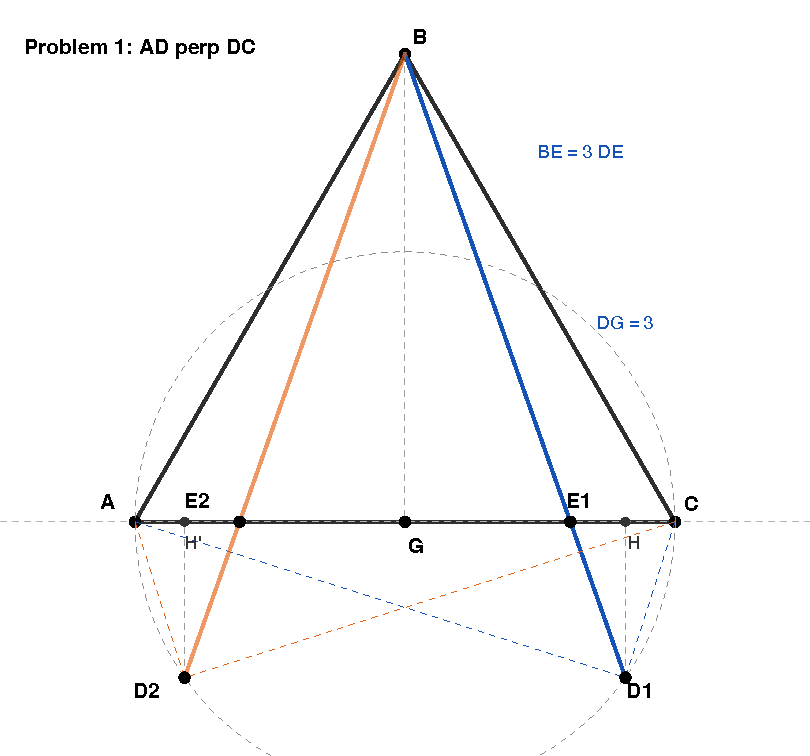
\includegraphics[width=0.68\linewidth]{figures/problem1.pdf}
\end{center}
\end{eduSoftBox}




\begin{eduSubQuestionItem}{几何法}
辅助线 + 相似 + 勾股。\end{eduSubQuestionItem}

\begin{eduSolutionBox}{几何法}
  \begingroup
  \setlength{\parskip}{2.5mm}
取 $G$ 为 $AC$ 中点。等边三角形边长为 $6$，所以 $AG=CG=3$，高 $BG=\sqrt{6^2-3^2}=3\sqrt3$。\par
因为 $AD\perp DC$，$\triangle ADC$ 是直角三角形，且 $G$ 是斜边 $AC$ 的中点，所以 $DG=\frac12AC=3$。\par
过 $D$ 作 $DH\perp AC$ 于 $H$。由于 $BG\perp AC$，所以 $BG\parallel DH$，$\angle EBG=\angle EDH$，$\angle EGB=\angle EHD$。\par
于是 $\triangle EBG\sim\triangle EDH$。又 $BE:DE=3:1$，相似三角形对应高也成 $3:1$，所以 $BG:DH=3:1$，即 $DH=\sqrt3$。\par
在直角三角形 $DGH$ 中，$DG=3$，$DH=\sqrt3$，因此 $GH=\sqrt{DG^2-DH^2}=\sqrt{9-3}=\sqrt6$。\par
从 $B$ 到 $D$，竖直方向一共跨过 $BG+DH=4\sqrt3$，水平方向跨过 $GH=\sqrt6$。\par
$BD=\sqrt{(4\sqrt3)^2+(\sqrt6)^2}=3\sqrt6$。\par
  \endgroup
  \vspace{2.5mm}
  {\color{edu-blue}\bfseries\small 本法小结}\par\vspace{1.5mm}
  \begin{eduBulletList}
    \item 几何法的核心不是一开始求 $E$，而是先用 $DG=3$ 和相似关系求出 $D$ 到 $AC$ 的距离。    \item 答案：$BD=3\sqrt6$。  \end{eduBulletList}
\end{eduSolutionBox}




\begin{eduSubQuestionItem}{向量法}
把比例点写成分点向量。\end{eduSubQuestionItem}

\begin{eduSolutionBox}{向量法}
  \begingroup
  \setlength{\parskip}{2.5mm}
以 $G$ 为原点式参照，令 $\vec{GE}=\mathbf e,\ \vec{GB}=\mathbf b$。其中 $\mathbf e$ 沿 $AC$，$\mathbf b$ 沿高，所以 $\mathbf e\perp\mathbf b$，$|\mathbf b|=3\sqrt3$。\par
本题 $E$ 在线段 $BD$ 上，且 $BE:DE=3:1$，所以从 $B$ 走到 $D$ 要经过 $E$ 后再走 $\frac13BE$。写成向量就是 $\vec{GD}=\mathbf b+\frac43(\mathbf e-\mathbf b)=\frac43\mathbf e-\frac13\mathbf b$。\par
由 $AD\perp DC$ 得 $DG=3$，因此 $9=|\vec{GD}|^2=\frac{16}{9}|\mathbf e|^2+\frac19|\mathbf b|^2$。这里没有交叉项，是因为 $\mathbf e\perp\mathbf b$。\par
代入 $|\mathbf b|^2=27$，得 $|\mathbf e|^2=\frac{27}{8}$。\par
又 $BE=\sqrt{|\mathbf e|^2+|\mathbf b|^2}$，且 $BD=\frac43BE$，所以 $BD=\frac43\sqrt{\frac{27}{8}+27}=3\sqrt6$。\par
  \endgroup
  \vspace{2.5mm}
  {\color{edu-blue}\bfseries\small 本法小结}\par\vspace{1.5mm}
  \begin{eduBulletList}
    \item 向量法把“比例点”直接翻译成 $\vec{GD}$，适合统一处理后面的直线分支。    \item 答案：$BD=3\sqrt6$。  \end{eduBulletList}
\end{eduSolutionBox}




\begin{eduSubQuestionItem}{建系法}
设 $E(x,0)$，把模型写成坐标。\end{eduSubQuestionItem}

\begin{eduSolutionBox}{建系法}
  \begingroup
  \setlength{\parskip}{2.5mm}
取 $G(0,0)$，$AC$ 为 $x$ 轴，则 $A(-3,0)$，$C(3,0)$，$B(0,3\sqrt3)$。设 $E(x,0)$，且本题 $-3\le x\le 3$。\par
因为 $E$ 在线段 $BD$ 上且 $BE=3DE$，所以 $D=B+\frac43(E-B)=(\frac43x,-\sqrt3)$。这个坐标式已经把比例条件完整用掉了。\par
$AD\perp DC$ 等价于 $DG=3$，所以 $(\frac43x)^2+(-\sqrt3)^2=9$，即 $\frac{16}{9}x^2+3=9$。\par
解得 $x^2=\frac{27}{8}$。这两个 $x$ 值都在 $[-3,3]$ 内，对应左右对称的两幅图，$BD$ 长度相同。\par
$BD=\frac43BE=\frac43\sqrt{x^2+27}=3\sqrt6$。\par
  \endgroup
  \vspace{2.5mm}
  {\color{edu-blue}\bfseries\small 本法小结}\par\vspace{1.5mm}
  \begin{eduBulletList}
    \item 建系法最稳定：先用比例写出 $D$，再把附加条件翻译成方程。    \item 答案：$BD=3\sqrt6$。  \end{eduBulletList}
\end{eduSolutionBox}



\clearpage
\eduSectionTitle{第2题：变式1}

\begin{eduProblemBlock}[第2题]
$AD=AC$，直线 $BD$ 和线段 $AC$ 交于点 $E$，且 $BE=3DE$，求 $BD$。

\end{eduProblemBlock}





\begin{eduAuxItem}{核心思路}
本题把 $AD\perp DC$ 换成 $AD=AC=6$，所以不能再用 $DG=3$。但是 $E$ 仍在线段 $AC$ 上，最后必须检查 $-3\le x\le3$。直线 $BD$ 允许两个分点分支，真正可行的是 $E$ 在线段 $BD$ 上这一支。
\end{eduAuxItem}




\begin{eduAuxItem}{思路导航}
仍取 $G$$\;\to\;$先判有效分支$\;\to\;$由相似求 $DH$$\;\to\;$用 $AD=6$ 求水平距离$\;\to\;$检查 $E$ 在线段 $AC$ 内\end{eduAuxItem}




\begin{eduSoftBox}
\eduSubTitle{Wolfram 插图}\begin{center}
  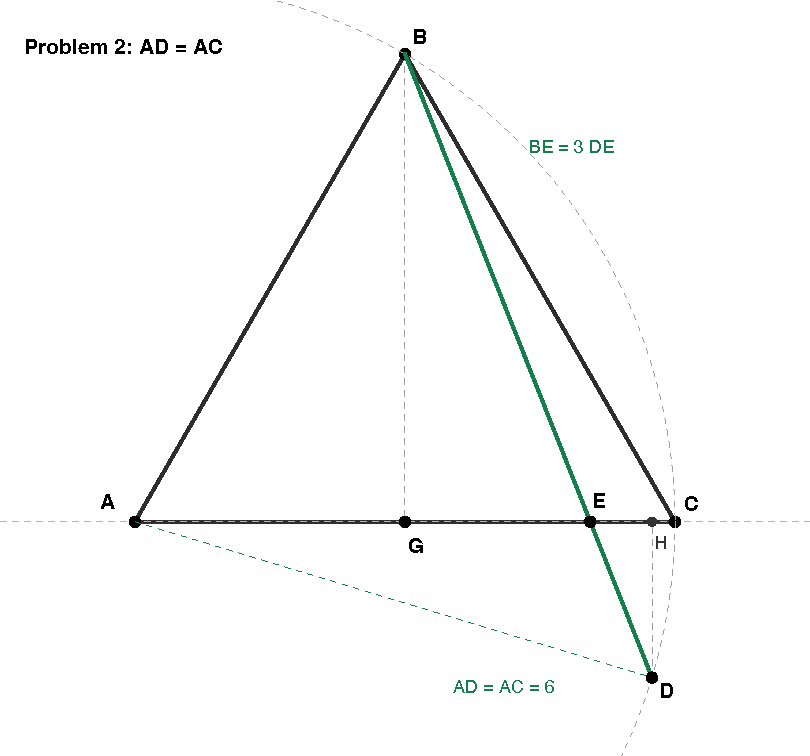
\includegraphics[width=0.68\linewidth]{figures/problem2.pdf}
\end{center}
\end{eduSoftBox}




\begin{eduSubQuestionItem}{几何法}
先判分支，再用 $AD=6$。\end{eduSubQuestionItem}

\begin{eduSolutionBox}{几何法}
  \begingroup
  \setlength{\parskip}{2.5mm}
取 $G$ 为 $AC$ 中点，仍有 $BG=3\sqrt3$。这一次 $AD=AC=6$ 只说明 $D$ 在以 $A$ 为圆心、半径 $6$ 的圆上，不能推出 $DG=3$。\par
先看分支。若 $D$ 在线段 $BE$ 上，则为了满足 $AD=6$ 会把 $E$ 推到线段 $AC$ 外；题目要求 $E$ 在线段 $AC$ 上，所以舍去。有效分支是 $E$ 在线段 $BD$ 上。\par
过 $D$ 作 $DH\perp AC$ 于 $H$。和第1题一样，$\triangle EBG\sim\triangle EDH$，由 $BE:DE=3:1$ 得 $BG:DH=3:1$，所以 $DH=\sqrt3$。\par
现在用的是 $AD=6$。在直角三角形 $ADH$ 中，$AH=\sqrt{AD^2-DH^2}=\sqrt{36-3}=\sqrt{33}$。\par
因为 $AG=3$，且有效图形中 $H$ 在 $G$ 的右侧，所以 $GH=AH-AG=\sqrt{33}-3$。\par
从 $B$ 到 $D$ 的竖直差仍是 $BG+DH=4\sqrt3$，水平差是 $GH=\sqrt{33}-3$。\par
$BD^2=(4\sqrt3)^2+(\sqrt{33}-3)^2=90-6\sqrt{33}$。\par
所以 $BD=\sqrt{90-6\sqrt{33}}$。\par
  \endgroup
  \vspace{2.5mm}
  {\color{edu-blue}\bfseries\small 本法小结}\par\vspace{1.5mm}
  \begin{eduBulletList}
    \item 和第1题相比，唯一换掉的是“求水平距离”的来源：第1题用 $DG=3$，本题用 $AD=6$。    \item 答案：$BD=\sqrt{90-6\sqrt{33}}$。  \end{eduBulletList}
\end{eduSolutionBox}




\begin{eduSubQuestionItem}{向量法}
同一个分点表达，换成 $AD=6$。\end{eduSubQuestionItem}

\begin{eduSolutionBox}{向量法}
  \begingroup
  \setlength{\parskip}{2.5mm}
令 $\vec{GE}=\mathbf e=x\mathbf u,\ \vec{GB}=\mathbf b$，其中 $\mathbf u$ 是 $AC$ 方向单位向量，$\mathbf e\perp\mathbf b$，$|\mathbf b|=3\sqrt3$，且 $\vec{GA}=-3\mathbf u$。\par
有效分支仍为 $E$ 在线段 $BD$ 上，所以 $\vec{GD}=\frac43\mathbf e-\frac13\mathbf b=\frac43x\mathbf u-\frac13\mathbf b$。\par
$AD=6$ 写成 $|\vec{GD}-\vec{GA}|=6$，即 $|\frac43x\mathbf u+3\mathbf u-\frac13\mathbf b|^2=36$。\par
利用垂直分量平方相加：$(\frac43x+3)^2+\frac19|\mathbf b|^2=36$，也就是 $(\frac43x+3)^2+3=36$。\par
解得 $x=\frac34(\sqrt{33}-3)$ 或 $x=-\frac34(\sqrt{33}+3)$。后者小于 $-3$，不在线段 $AC$ 内，舍去。\par
有效根代回 $BD=\frac43BE=\frac43\sqrt{x^2+27}$，得 $BD^2=90-6\sqrt{33}$。\par
因此 $BD=\sqrt{90-6\sqrt{33}}$。\par
  \endgroup
  \vspace{2.5mm}
  {\color{edu-blue}\bfseries\small 本法小结}\par\vspace{1.5mm}
  \begin{eduBulletList}
    \item 向量法里舍根最清楚：根是否满足 $-3\le x\le3$，一看就能判定。    \item 答案：$BD=\sqrt{90-6\sqrt{33}}$。  \end{eduBulletList}
\end{eduSolutionBox}




\begin{eduSubQuestionItem}{建系法}
坐标最方便检查舍根。\end{eduSubQuestionItem}

\begin{eduSolutionBox}{建系法}
  \begingroup
  \setlength{\parskip}{2.5mm}
仍取 $G(0,0)$，$A(-3,0)$，$C(3,0)$，$B(0,3\sqrt3)$，设 $E(x,0)$。\par
先取有效分支 $E$ 在线段 $BD$ 上，于是 $D=(\frac43x,-\sqrt3)$。这一步和第1题完全相同。\par
由 $AD=6$，得 $(\frac43x+3)^2+(-\sqrt3)^2=36$，即 $(\frac43x+3)^2+3=36$。\par
解得 $x=\frac34(\sqrt{33}-3)$ 或 $x=-\frac34(\sqrt{33}+3)$。由于 $E$ 在线段 $AC$ 上，必须 $-3\le x\le3$，所以只保留 $x=\frac34(\sqrt{33}-3)$。\par
于是 $BD=\frac43BE=\frac43\sqrt{x^2+27}$。代入有效根并化简，得 $BD=\sqrt{90-6\sqrt{33}}$。\par
如果尝试另一分点分支，也会在 $x$ 的范围检查中被排除，因此本题只有一个答案。\par
  \endgroup
  \vspace{2.5mm}
  {\color{edu-blue}\bfseries\small 本法小结}\par\vspace{1.5mm}
  \begin{eduBulletList}
    \item 建系法的关键不是方程难，而是方程解完以后必须检查 $E$ 是否仍在线段 $AC$ 上。    \item 答案：$BD=\sqrt{90-6\sqrt{33}}$。  \end{eduBulletList}
\end{eduSolutionBox}



\clearpage
\eduSectionTitle{第3题：变式2}

\begin{eduProblemBlock}[第3题]
$AD\perp DC$，直线 $BD$ 和直线 $AC$ 交于点 $E$，且 $BE=3DE$，求 $BD$。

\end{eduProblemBlock}





\begin{eduAuxItem}{核心思路}
本题和第1题一样有 $AD\perp DC$，所以仍有 $DG=3$。变化在“直线 $BD$ 和直线 $AC$”：$E$ 不一定夹在 $B,D$ 之间，也不一定在线段 $AC$ 内。因此两个分点分支都要算，再按直线条件保留。
\end{eduAuxItem}




\begin{eduAuxItem}{思路导航}
保留 $DG=3$$\;\to\;$列两个分点分支$\;\to\;$分别求 $DH,GH$ 或 $x$$\;\to\;$判断是否只在线段外$\;\to\;$直线条件允许则保留\end{eduAuxItem}




\begin{eduSoftBox}
\eduSubTitle{Wolfram 插图}\begin{center}
  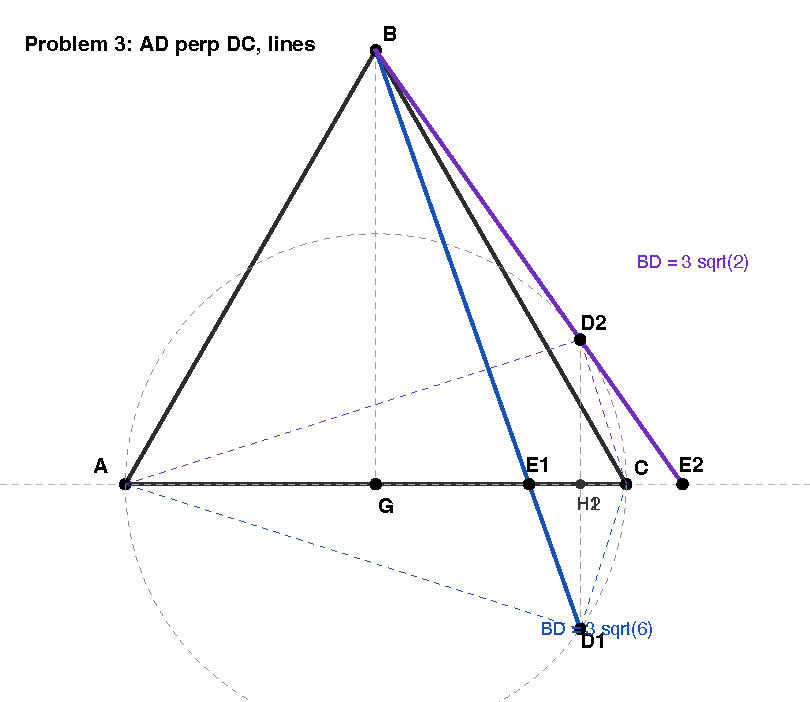
\includegraphics[width=0.70\linewidth]{figures/problem3.pdf}
\end{center}
\end{eduSoftBox}




\begin{eduSubQuestionItem}{几何法}
直线条件带来两个分支。\end{eduSubQuestionItem}

\begin{eduSolutionBox}{几何法}
  \begingroup
  \setlength{\parskip}{2.5mm}
$AD\perp DC$ 仍然给出 $DG=3$，并且 $BG=3\sqrt3$ 不变。\par
分支一：$E$ 在线段 $BD$ 上。这时与第1题完全相同，由相似得 $DH=\sqrt3$，再由 $DG=3$ 得 $GH=\sqrt6$。竖直差为 $BG+DH=4\sqrt3$，所以 $BD=3\sqrt6$。\par
分支二：$D$ 在线段 $BE$ 上。此时 $D$ 在 $B$ 与 $E$ 之间，作 $DH\perp AC$ 后，仍由相似比 $BE:DE=3:1$ 得 $DH=\sqrt3$。\par
由于 $DG=3$，仍有 $GH=\sqrt{9-3}=\sqrt6$。但这一次 $D$ 在 $B$ 下方、$AC$ 上方，竖直差是 $BG-DH=2\sqrt3$。\par
所以第二个长度 $BD=\sqrt{(2\sqrt3)^2+(\sqrt6)^2}=3\sqrt2$。这个分支会让 $E$ 落在 $AC$ 的延长线上，但题目说的是直线 $AC$，所以不能舍。\par
  \endgroup
  \vspace{2.5mm}
  {\color{edu-blue}\bfseries\small 本法小结}\par\vspace{1.5mm}
  \begin{eduBulletList}
    \item 本题最容易错在把“直线”看成“线段”，从而漏掉 $3\sqrt2$。    \item 答案：$BD=3\sqrt6$ 或 $3\sqrt2$。  \end{eduBulletList}
\end{eduSolutionBox}




\begin{eduSubQuestionItem}{向量法}
两个分点表达都要取。\end{eduSubQuestionItem}

\begin{eduSolutionBox}{向量法}
  \begingroup
  \setlength{\parskip}{2.5mm}
仍令 $\vec{GE}=\mathbf e,\ \vec{GB}=\mathbf b$，其中 $\mathbf e\perp\mathbf b$，$|\mathbf b|^2=27$，且由 $AD\perp DC$ 得 $|\vec{GD}|=3$。\par
分支一：$E$ 在线段 $BD$ 上，$\vec{GD}=\frac43\mathbf e-\frac13\mathbf b$。代入 $|\vec{GD}|=3$，得 $\frac{16}{9}|\mathbf e|^2+3=9$，即 $|\mathbf e|^2=\frac{27}{8}$，所以 $BD=3\sqrt6$。\par
分支二：$D$ 在线段 $BE$ 上，$\vec{GD}=\frac23\mathbf e+\frac13\mathbf b$。代入 $|\vec{GD}|=3$，得 $\frac49|\mathbf e|^2+3=9$，即 $|\mathbf e|^2=\frac{27}{2}$。\par
这一支中 $BD=\frac23BE$，于是 $BD=\frac23\sqrt{|\mathbf e|^2+|\mathbf b|^2}=\frac23\sqrt{\frac{27}{2}+27}=3\sqrt2$。\par
因为本题是直线 $BD$ 与直线 $AC$，两个分支都合法。\par
  \endgroup
  \vspace{2.5mm}
  {\color{edu-blue}\bfseries\small 本法小结}\par\vspace{1.5mm}
  \begin{eduBulletList}
    \item 向量法特别适合这题，因为两个分支只差一个分点表达式。    \item 答案：$BD=3\sqrt6$ 或 $3\sqrt2$。  \end{eduBulletList}
\end{eduSolutionBox}




\begin{eduSubQuestionItem}{建系法}
两个坐标分支分别代入 $DG=3$。\end{eduSubQuestionItem}

\begin{eduSolutionBox}{建系法}
  \begingroup
  \setlength{\parskip}{2.5mm}
仍设 $G(0,0)$，$B(0,3\sqrt3)$，$E(x,0)$。直线条件下，$x$ 不必限制在 $[-3,3]$。\par
分支一：$E$ 在线段 $BD$ 上，$D=(\frac43x,-\sqrt3)$。代入 $DG=3$ 得 $\frac{16}{9}x^2+3=9$，所以 $x^2=\frac{27}{8}$，进而 $BD=3\sqrt6$。\par
分支二：$D$ 在线段 $BE$ 上，$D=(\frac23x,\sqrt3)$。代入 $DG=3$ 得 $\frac49x^2+3=9$，所以 $x^2=\frac{27}{2}$，进而 $BD=3\sqrt2$。\par
第二分支的 $|x|>3$，如果是线段 $AC$ 要舍；但这里是直线 $AC$，保留。\par
  \endgroup
  \vspace{2.5mm}
  {\color{edu-blue}\bfseries\small 本法小结}\par\vspace{1.5mm}
  \begin{eduBulletList}
    \item 坐标法把“直线”和“线段”的区别落实为 $x$ 是否必须落在 $[-3,3]$。    \item 答案：$BD=3\sqrt6$ 或 $3\sqrt2$。  \end{eduBulletList}
\end{eduSolutionBox}



\clearpage
\eduSectionTitle{第4题：变式3}

\begin{eduProblemBlock}[第4题]
$BD\perp DC$，直线 $BD$ 和线段 $AC$ 交于点 $E$，且 $BE=3DE$，求 $BD$。

\end{eduProblemBlock}





\begin{eduAuxItem}{核心思路}
本题最容易误套第1题：条件是 $BD\perp DC$，不是 $AD\perp DC$，所以没有 $DG=3$。不过 $E$ 仍在线段 $AC$ 上，这会排除一部分分支。有效做法是先用比例写出 $D$ 的位置，再把 $BD\perp DC$ 翻译成几何乘积或坐标点积。
\end{eduAuxItem}




\begin{eduAuxItem}{思路导航}
不能用 $DG=3$$\;\to\;$判断有效分支为 $D$ 在线段 $BE$ 上$\;\to\;$设 $GH=t$ 或 $E(x,0)$$\;\to\;$用 $BD\perp DC$ 建方程$\;\to\;$检查有效根\end{eduAuxItem}




\begin{eduSoftBox}
\eduSubTitle{Wolfram 插图}\begin{center}
  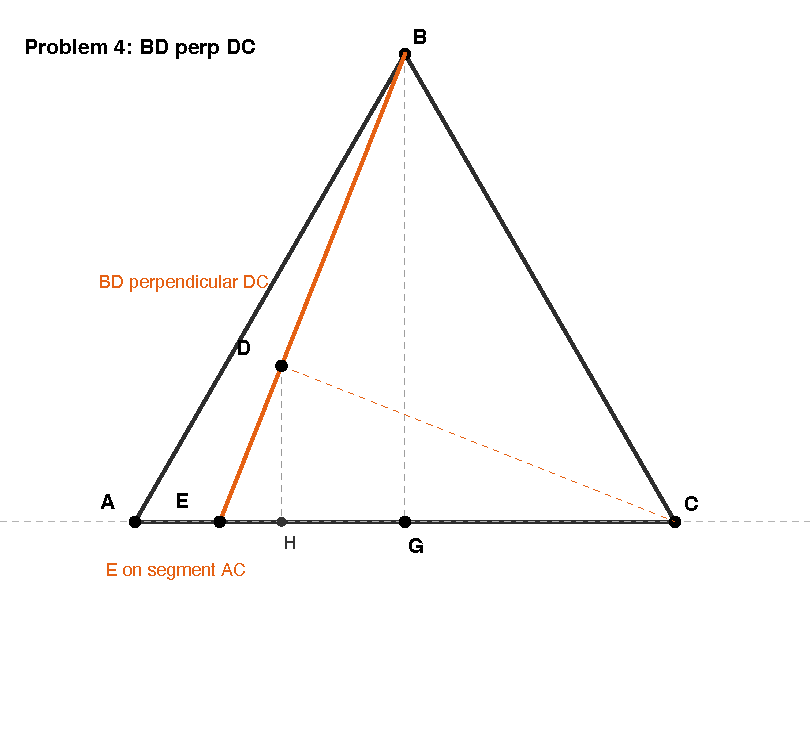
\includegraphics[width=0.68\linewidth]{figures/problem4.pdf}
\end{center}
\end{eduSoftBox}




\begin{eduSubQuestionItem}{几何法}
这次不能用 $DG=3$，改用 $BD\perp DC$。\end{eduSubQuestionItem}

\begin{eduSolutionBox}{几何法}
  \begingroup
  \setlength{\parskip}{2.5mm}
先不要写 $DG=3$，因为本题没有 $AD\perp DC$。由线段 $AC$ 的限制检查分支，可行的是 $D$ 在线段 $BE$ 上。\par
作 $DH\perp AC$。由 $\triangle EBG\sim\triangle EDH$ 和 $BE:DE=3:1$，仍得 $BG:DH=3:1$，所以 $DH=\sqrt3$。此时 $D$ 在 $AC$ 上方。\par
设 $H$ 在 $G$ 左侧，$GH=t$。从 $D$ 看向 $B$，水平差为 $t$，竖直差为 $BG-DH=2\sqrt3$。\par
从 $D$ 看向 $C$，水平差为 $CG+GH=3+t$，竖直差为 $DH=\sqrt3$。\par
因为 $BD\perp DC$，两个方向的斜率乘积为 $-1$；等价地，水平差乘积等于竖直差乘积，所以 $t(3+t)=2\sqrt3\cdot\sqrt3=6$。\par
解得 $t=\frac{\sqrt{33}-3}{2}$。\par
于是 $BD^2=t^2+(2\sqrt3)^2=\frac{45-3\sqrt{33}}{2}$。\par
所以 $BD=\sqrt{\frac{45-3\sqrt{33}}{2}}$。\par
  \endgroup
  \vspace{2.5mm}
  {\color{edu-blue}\bfseries\small 本法小结}\par\vspace{1.5mm}
  \begin{eduBulletList}
    \item 本题的关键是换垂直对象：从“斜边中线”模型切到“垂直方向点积/斜率”模型。    \item 答案：$BD=\sqrt{\frac{45-3\sqrt{33}}{2}}$。  \end{eduBulletList}
\end{eduSolutionBox}




\begin{eduSubQuestionItem}{向量法}
垂直写成点积为零。\end{eduSubQuestionItem}

\begin{eduSolutionBox}{向量法}
  \begingroup
  \setlength{\parskip}{2.5mm}
令 $\vec{GE}=x\mathbf u,\ \vec{GB}=\mathbf b$，其中 $\mathbf u$ 沿 $AC$，$|\mathbf b|=3\sqrt3$，$\vec{GC}=3\mathbf u$。\par
先试 $E$ 在线段 $BD$ 上的分支：$\vec{GD}=\frac43x\mathbf u-\frac13\mathbf b$。把 $BD\perp DC$ 写成 $(\vec{GB}-\vec{GD})\cdot(\vec{GC}-\vec{GD})=0$，会得到判别式小于 $0$ 的方程，因此无实数解。\par
有效分支为 $D$ 在线段 $BE$ 上：$\vec{GD}=\frac23x\mathbf u+\frac13\mathbf b$。\par
代入点积方程 $(\vec{GB}-\vec{GD})\cdot(\vec{GC}-\vec{GD})=0$，利用 $\mathbf u\perp\mathbf b$，得到 $4x^2-18x-54=0$。\par
解得 $x=\frac{9\pm3\sqrt{33}}4$。线段 $AC$ 要求 $-3\le x\le3$，所以取 $x=\frac{9-3\sqrt{33}}4$。\par
此时 $BD=\frac23BE=\frac23\sqrt{x^2+27}$，化简得 $BD^2=\frac{45-3\sqrt{33}}{2}$。\par
所以 $BD=\sqrt{\frac{45-3\sqrt{33}}{2}}$。\par
  \endgroup
  \vspace{2.5mm}
  {\color{edu-blue}\bfseries\small 本法小结}\par\vspace{1.5mm}
  \begin{eduBulletList}
    \item 向量法中，垂直条件最干净的表达就是点积为 $0$，比斜率更不容易漏符号。    \item 答案：$BD=\sqrt{\frac{45-3\sqrt{33}}{2}}$。  \end{eduBulletList}
\end{eduSolutionBox}




\begin{eduSubQuestionItem}{建系法}
坐标直接判有效根。\end{eduSubQuestionItem}

\begin{eduSolutionBox}{建系法}
  \begingroup
  \setlength{\parskip}{2.5mm}
设 $G(0,0)$，$B(0,3\sqrt3)$，$C(3,0)$，$E(x,0)$，并且因为 $E$ 在线段 $AC$ 上，要有 $-3\le x\le3$。\par
先检查分支。若 $E$ 在线段 $BD$ 上，则 $D=(\frac43x,-\sqrt3)$，代入 $(B-D)\cdot(C-D)=0$ 得 $4x^2-9x+27=0$，没有实数解。\par
因此取 $D$ 在线段 $BE$ 上的分支：$D=(\frac23x,\sqrt3)$。\par
$BD\perp DC$ 写成 $(B-D)\cdot(C-D)=0$，即 $(-\frac23x,2\sqrt3)\cdot(3-\frac23x,-\sqrt3)=0$。\par
展开得 $4x^2-18x-54=0$，所以 $x=\frac{9\pm3\sqrt{33}}4$。\par
根 $x=\frac{9+3\sqrt{33}}4$ 大于 $3$，不在线段 $AC$ 上，舍去；有效根为 $x=\frac{9-3\sqrt{33}}4$。\par
$BD=\frac23BE=\frac23\sqrt{x^2+27}=\sqrt{\frac{45-3\sqrt{33}}{2}}$。\par
  \endgroup
  \vspace{2.5mm}
  {\color{edu-blue}\bfseries\small 本法小结}\par\vspace{1.5mm}
  \begin{eduBulletList}
    \item 建系法把本题所有限制都落到三件事：分支、点积、范围。    \item 答案：$BD=\sqrt{\frac{45-3\sqrt{33}}{2}}$。  \end{eduBulletList}
\end{eduSolutionBox}



\clearpage
\eduSectionTitle{总答案与方法对照}

\begin{eduSummaryBlock}{\eduIconCheck}{四题答案}
\begin{eduPlainList}
  \item 第1题：$BD=3\sqrt6$  \item 第2题：$BD=\sqrt{90-6\sqrt{33}}$  \item 第3题：$BD=3\sqrt6$ 或 $3\sqrt2$  \item 第4题：$BD=\sqrt{\frac{45-3\sqrt{33}}{2}}$\end{eduPlainList}
\end{eduSummaryBlock}




\begin{eduSummaryBlock}{\eduIconPin}{三种方法区别}
\begin{eduBulletList}
  \item 几何法：最能看出图形结构，重点是辅助线、相似和勾股。  \item 向量法：最能表达分点关系，尤其适合处理 $E$ 在线段 $BD$ 上和 $D$ 在线段 $BE$ 上两个分支。  \item 建系法：最适合处理变式和检查舍根，把线段 $AC$ 的限制落实为 $-3\le x\le3$。\end{eduBulletList}
\end{eduSummaryBlock}




\begin{eduMistakeBox}
\eduSubTitle{变式1条件}变式1是 $AD=AC$，不是 $AD=DC$。这会改变 $D$ 的轨迹，不能再把它当作垂直平分线问题。
\end{eduMistakeBox}




\begin{eduMistakeBox}
\eduSubTitle{四题都要先判分支}$BE=3DE$ 不是自动等于 $BD=\frac43BE$。如果题目说直线 $BD$，还要检查 $D$ 在线段 $BE$ 上的分支，此时 $BD=\frac23BE$。
\end{eduMistakeBox}



\clearpage
\eduSectionTitle{教师备注}

\begin{eduAuxItem}{核心思路}
这份讲义按四道题拆开，每道题都给出三种方法。讲课建议不要一次性讲完所有代数细节：先用第1题建立 $B,G,E,D$ 小模型，再让学生在第2-4题中练“分支 + 范围检查”。
\end{eduAuxItem}


\begin{eduTeacherNote}
  \textbf{训练目标：}四题三法对照，训练共同模型与分支检查\par
  \textbf{预期卡点：}学生知道建系但不知道为什么要先取G
\end{eduTeacherNote}


\end{document}
